\pdfoptionpdfminorversion=7
\documentclass{beamer}

\mode<presentation>
{
  \usetheme{Madrid}       % or try default, Darmstadt, Warsaw, ...
  \usecolortheme{default} % or try albatross, beaver, crane, ...
  \usefonttheme{serif}    % or try default, structurebold, ...
  \setbeamertemplate{navigation symbols}{}
  \setbeamertemplate{caption}[numbered]
}

\usepackage{amsmath}
\usepackage[utf8x]{inputenc}
\usepackage{listings}
\usepackage{graphicx}
\usepackage{lmodern}

\usetheme{default}

\title{Proyecto de titulo I}
\author{Yerko Zec}
\institute[]{FI - UNAB}
\date{2019/09/03}


\begin{document}

\begin{frame}[plain]
  \titlepage
\end{frame}

\addtocounter{framenumber}{-1}

\begin{frame}{Sorting algorithms}
\begin{itemize}
 \item Se estudío metodos de detección de contactos
 \item TLS(busqueda de dos niveles) la cual se divide en dos fases, la busqueda de vecinos y luego la detecion de contacto entre particulas vecinas
 \item Para la detección del vecindario se utilizaran 2 algoritmos DESS (Performance O(N**{2})) y  NBS (Performance O(N)).
 \item DESS performance es insensible ante variación de tamaño entre particulas.
 \item NBS reduccion de performance significativo con una alta variación entre tamaño de particulas.
\end{itemize}
\end{frame}

\begin{frame}{Contact detection}
\begin{itemize}
 \item Se utilizó el algoritmo de detección de contacto SLM(Shortest Link Method) debido a que tiene una nuevo enfoque para encontrar CP(Common Plane).
 \item Este metodo tiene la restricción de ser solo para particulas convexas.

 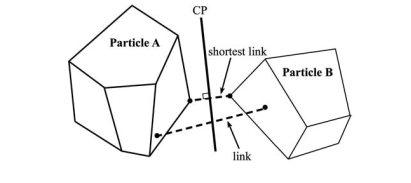
\includegraphics[width=0.5\linewidth]{CP}
\end{itemize}
\end{frame}

\begin{frame}{Problemas}
 \begin{itemize}
  \item Ligeros problemas de comprención.
  \item Administracion de tiempos.
 \end{itemize}
\end{frame}


\begin{frame}{ToDo}
\begin{itemize}
 \item Lectura de nuevo paper sobre nuevos algoritmos de detección de contacto.
 \item Definicion hora minima de trabajo diario. 
\end{itemize}
\end{frame}

\medskip
\bibliographystyle{plain}
\bibliography{/home/yerkozec/Desktop/pt/memoria/Referencia}

\end{document}
